\documentclass[]{article}
\usepackage{lmodern}
\usepackage{amssymb,amsmath}
\usepackage{ifxetex,ifluatex}
\usepackage{fixltx2e} % provides \textsubscript
\ifnum 0\ifxetex 1\fi\ifluatex 1\fi=0 % if pdftex
  \usepackage[T1]{fontenc}
  \usepackage[utf8]{inputenc}
\else % if luatex or xelatex
  \ifxetex
    \usepackage{mathspec}
  \else
    \usepackage{fontspec}
  \fi
  \defaultfontfeatures{Ligatures=TeX,Scale=MatchLowercase}
\fi
% use upquote if available, for straight quotes in verbatim environments
\IfFileExists{upquote.sty}{\usepackage{upquote}}{}
% use microtype if available
\IfFileExists{microtype.sty}{%
\usepackage{microtype}
\UseMicrotypeSet[protrusion]{basicmath} % disable protrusion for tt fonts
}{}
\usepackage[margin=1in]{geometry}
\usepackage{hyperref}
\hypersetup{unicode=true,
            pdftitle={Lab1: Demo RMarkdown \& EDA},
            pdfauthor={Silvia Montagna},
            pdfborder={0 0 0},
            breaklinks=true}
\urlstyle{same}  % don't use monospace font for urls
\usepackage{color}
\usepackage{fancyvrb}
\newcommand{\VerbBar}{|}
\newcommand{\VERB}{\Verb[commandchars=\\\{\}]}
\DefineVerbatimEnvironment{Highlighting}{Verbatim}{commandchars=\\\{\}}
% Add ',fontsize=\small' for more characters per line
\usepackage{framed}
\definecolor{shadecolor}{RGB}{248,248,248}
\newenvironment{Shaded}{\begin{snugshade}}{\end{snugshade}}
\newcommand{\KeywordTok}[1]{\textcolor[rgb]{0.13,0.29,0.53}{\textbf{#1}}}
\newcommand{\DataTypeTok}[1]{\textcolor[rgb]{0.13,0.29,0.53}{#1}}
\newcommand{\DecValTok}[1]{\textcolor[rgb]{0.00,0.00,0.81}{#1}}
\newcommand{\BaseNTok}[1]{\textcolor[rgb]{0.00,0.00,0.81}{#1}}
\newcommand{\FloatTok}[1]{\textcolor[rgb]{0.00,0.00,0.81}{#1}}
\newcommand{\ConstantTok}[1]{\textcolor[rgb]{0.00,0.00,0.00}{#1}}
\newcommand{\CharTok}[1]{\textcolor[rgb]{0.31,0.60,0.02}{#1}}
\newcommand{\SpecialCharTok}[1]{\textcolor[rgb]{0.00,0.00,0.00}{#1}}
\newcommand{\StringTok}[1]{\textcolor[rgb]{0.31,0.60,0.02}{#1}}
\newcommand{\VerbatimStringTok}[1]{\textcolor[rgb]{0.31,0.60,0.02}{#1}}
\newcommand{\SpecialStringTok}[1]{\textcolor[rgb]{0.31,0.60,0.02}{#1}}
\newcommand{\ImportTok}[1]{#1}
\newcommand{\CommentTok}[1]{\textcolor[rgb]{0.56,0.35,0.01}{\textit{#1}}}
\newcommand{\DocumentationTok}[1]{\textcolor[rgb]{0.56,0.35,0.01}{\textbf{\textit{#1}}}}
\newcommand{\AnnotationTok}[1]{\textcolor[rgb]{0.56,0.35,0.01}{\textbf{\textit{#1}}}}
\newcommand{\CommentVarTok}[1]{\textcolor[rgb]{0.56,0.35,0.01}{\textbf{\textit{#1}}}}
\newcommand{\OtherTok}[1]{\textcolor[rgb]{0.56,0.35,0.01}{#1}}
\newcommand{\FunctionTok}[1]{\textcolor[rgb]{0.00,0.00,0.00}{#1}}
\newcommand{\VariableTok}[1]{\textcolor[rgb]{0.00,0.00,0.00}{#1}}
\newcommand{\ControlFlowTok}[1]{\textcolor[rgb]{0.13,0.29,0.53}{\textbf{#1}}}
\newcommand{\OperatorTok}[1]{\textcolor[rgb]{0.81,0.36,0.00}{\textbf{#1}}}
\newcommand{\BuiltInTok}[1]{#1}
\newcommand{\ExtensionTok}[1]{#1}
\newcommand{\PreprocessorTok}[1]{\textcolor[rgb]{0.56,0.35,0.01}{\textit{#1}}}
\newcommand{\AttributeTok}[1]{\textcolor[rgb]{0.77,0.63,0.00}{#1}}
\newcommand{\RegionMarkerTok}[1]{#1}
\newcommand{\InformationTok}[1]{\textcolor[rgb]{0.56,0.35,0.01}{\textbf{\textit{#1}}}}
\newcommand{\WarningTok}[1]{\textcolor[rgb]{0.56,0.35,0.01}{\textbf{\textit{#1}}}}
\newcommand{\AlertTok}[1]{\textcolor[rgb]{0.94,0.16,0.16}{#1}}
\newcommand{\ErrorTok}[1]{\textcolor[rgb]{0.64,0.00,0.00}{\textbf{#1}}}
\newcommand{\NormalTok}[1]{#1}
\usepackage{graphicx,grffile}
\makeatletter
\def\maxwidth{\ifdim\Gin@nat@width>\linewidth\linewidth\else\Gin@nat@width\fi}
\def\maxheight{\ifdim\Gin@nat@height>\textheight\textheight\else\Gin@nat@height\fi}
\makeatother
% Scale images if necessary, so that they will not overflow the page
% margins by default, and it is still possible to overwrite the defaults
% using explicit options in \includegraphics[width, height, ...]{}
\setkeys{Gin}{width=\maxwidth,height=\maxheight,keepaspectratio}
\IfFileExists{parskip.sty}{%
\usepackage{parskip}
}{% else
\setlength{\parindent}{0pt}
\setlength{\parskip}{6pt plus 2pt minus 1pt}
}
\setlength{\emergencystretch}{3em}  % prevent overfull lines
\providecommand{\tightlist}{%
  \setlength{\itemsep}{0pt}\setlength{\parskip}{0pt}}
\setcounter{secnumdepth}{0}
% Redefines (sub)paragraphs to behave more like sections
\ifx\paragraph\undefined\else
\let\oldparagraph\paragraph
\renewcommand{\paragraph}[1]{\oldparagraph{#1}\mbox{}}
\fi
\ifx\subparagraph\undefined\else
\let\oldsubparagraph\subparagraph
\renewcommand{\subparagraph}[1]{\oldsubparagraph{#1}\mbox{}}
\fi

%%% Use protect on footnotes to avoid problems with footnotes in titles
\let\rmarkdownfootnote\footnote%
\def\footnote{\protect\rmarkdownfootnote}

%%% Change title format to be more compact
\usepackage{titling}

% Create subtitle command for use in maketitle
\newcommand{\subtitle}[1]{
  \posttitle{
    \begin{center}\large#1\end{center}
    }
}

\setlength{\droptitle}{-2em}
  \title{Lab1: Demo RMarkdown \& EDA}
  \pretitle{\vspace{\droptitle}\centering\huge}
  \posttitle{\par}
\subtitle{MAT43 Statistical Machine Learning}
  \author{Silvia Montagna}
  \preauthor{\centering\large\emph}
  \postauthor{\par}
  \predate{\centering\large\emph}
  \postdate{\par}
  \date{03/06/2018}


\begin{document}
\maketitle

\section{Exercise 8 from ISLR Chapter
2}\label{exercise-8-from-islr-chapter-2}

The following illustrate commands for exploring this exercise using R
and various packages for the \texttt{College} data. The \texttt{College}
dataset contains a number of variables for 777 different universities
and colleges in the US.

\subsubsection{Libraries}\label{libraries}

Try to load the \texttt{ISLR} library

\begin{Shaded}
\begin{Highlighting}[]
\KeywordTok{library}\NormalTok{(ISLR)}
\end{Highlighting}
\end{Shaded}

If it is not available you will need to install the library from CRAN.
Click on \emph{Packages} then \emph{Install}. Enter the package name
then click on the Install button.

You can also install from the console/command line using
\texttt{install.packages("ISLR")}.

Ready?

\subsubsection{Getting the College data}\label{getting-the-college-data}

Next we will need to load the dataset. This is part of the library so we
will not need to read it in using \texttt{read.csv} but rather we will
use the \texttt{data} function to load it from the library.

\begin{Shaded}
\begin{Highlighting}[]
\KeywordTok{data}\NormalTok{(College)}
\end{Highlighting}
\end{Shaded}

This loads the dataframe \texttt{College}. Note you can always see the
content of any \texttt{R} object by simply typing its name, e.g.~by
typing \texttt{College} in the \texttt{R} console.

For information about the variables, read the text or enter

\begin{Shaded}
\begin{Highlighting}[]
\KeywordTok{help}\NormalTok{(College)}
\end{Highlighting}
\end{Shaded}

The info will appear in the \texttt{help} tab.

To explore the data, you can use the command \texttt{View(College)}.
This will open a new tab, where you may scroll left and right to look at
the rows and columns. In the \texttt{View} you should see that the first
column is the College/University name. These can be extracted using
\texttt{rownames(College)}. Let's print out the first 5

\begin{Shaded}
\begin{Highlighting}[]
\KeywordTok{rownames}\NormalTok{(College)[}\DecValTok{1}\OperatorTok{:}\DecValTok{5}\NormalTok{]}
\end{Highlighting}
\end{Shaded}

\begin{verbatim}
## [1] "Abilene Christian University" "Adelphi University"          
## [3] "Adrian College"               "Agnes Scott College"         
## [5] "Alaska Pacific University"
\end{verbatim}

\subsubsection{Summary}\label{summary}

We can pull up basic information about the variables using the
\texttt{summary()} function

\begin{Shaded}
\begin{Highlighting}[]
\KeywordTok{summary}\NormalTok{(College)}
\end{Highlighting}
\end{Shaded}

\begin{verbatim}
##  Private        Apps           Accept          Enroll       Top10perc    
##  No :212   Min.   :   81   Min.   :   72   Min.   :  35   Min.   : 1.00  
##  Yes:565   1st Qu.:  776   1st Qu.:  604   1st Qu.: 242   1st Qu.:15.00  
##            Median : 1558   Median : 1110   Median : 434   Median :23.00  
##            Mean   : 3002   Mean   : 2019   Mean   : 780   Mean   :27.56  
##            3rd Qu.: 3624   3rd Qu.: 2424   3rd Qu.: 902   3rd Qu.:35.00  
##            Max.   :48094   Max.   :26330   Max.   :6392   Max.   :96.00  
##    Top25perc      F.Undergrad     P.Undergrad         Outstate    
##  Min.   :  9.0   Min.   :  139   Min.   :    1.0   Min.   : 2340  
##  1st Qu.: 41.0   1st Qu.:  992   1st Qu.:   95.0   1st Qu.: 7320  
##  Median : 54.0   Median : 1707   Median :  353.0   Median : 9990  
##  Mean   : 55.8   Mean   : 3700   Mean   :  855.3   Mean   :10441  
##  3rd Qu.: 69.0   3rd Qu.: 4005   3rd Qu.:  967.0   3rd Qu.:12925  
##  Max.   :100.0   Max.   :31643   Max.   :21836.0   Max.   :21700  
##    Room.Board       Books           Personal         PhD        
##  Min.   :1780   Min.   :  96.0   Min.   : 250   Min.   :  8.00  
##  1st Qu.:3597   1st Qu.: 470.0   1st Qu.: 850   1st Qu.: 62.00  
##  Median :4200   Median : 500.0   Median :1200   Median : 75.00  
##  Mean   :4358   Mean   : 549.4   Mean   :1341   Mean   : 72.66  
##  3rd Qu.:5050   3rd Qu.: 600.0   3rd Qu.:1700   3rd Qu.: 85.00  
##  Max.   :8124   Max.   :2340.0   Max.   :6800   Max.   :103.00  
##     Terminal       S.F.Ratio      perc.alumni        Expend     
##  Min.   : 24.0   Min.   : 2.50   Min.   : 0.00   Min.   : 3186  
##  1st Qu.: 71.0   1st Qu.:11.50   1st Qu.:13.00   1st Qu.: 6751  
##  Median : 82.0   Median :13.60   Median :21.00   Median : 8377  
##  Mean   : 79.7   Mean   :14.09   Mean   :22.74   Mean   : 9660  
##  3rd Qu.: 92.0   3rd Qu.:16.50   3rd Qu.:31.00   3rd Qu.:10830  
##  Max.   :100.0   Max.   :39.80   Max.   :64.00   Max.   :56233  
##    Grad.Rate     
##  Min.   : 10.00  
##  1st Qu.: 53.00  
##  Median : 65.00  
##  Mean   : 65.46  
##  3rd Qu.: 78.00  
##  Max.   :118.00
\end{verbatim}

\subsubsection{Data dimension}\label{data-dimension}

How many observations and variables are in the dataframe?

\begin{Shaded}
\begin{Highlighting}[]
\NormalTok{d =}\StringTok{ }\KeywordTok{dim}\NormalTok{(College)}
\end{Highlighting}
\end{Shaded}

Suppose we want to refer to those numbers in the text. We can extract
them using n = 777 and d = 18. Look at the Rmd code to see how we
extracted them.

\subsubsection{Scatter plot matrices}\label{scatter-plot-matrices}

This \texttt{base} \texttt{R} version of scatter plot matrices is
obtained using the \texttt{pairs} function to plot all variables versus
each other. We can use subsetting of columns of the dataframe to look at
the first 5 columns.

\begin{Shaded}
\begin{Highlighting}[]
\KeywordTok{pairs}\NormalTok{(College[, }\DecValTok{1}\OperatorTok{:}\DecValTok{5}\NormalTok{])}
\end{Highlighting}
\end{Shaded}

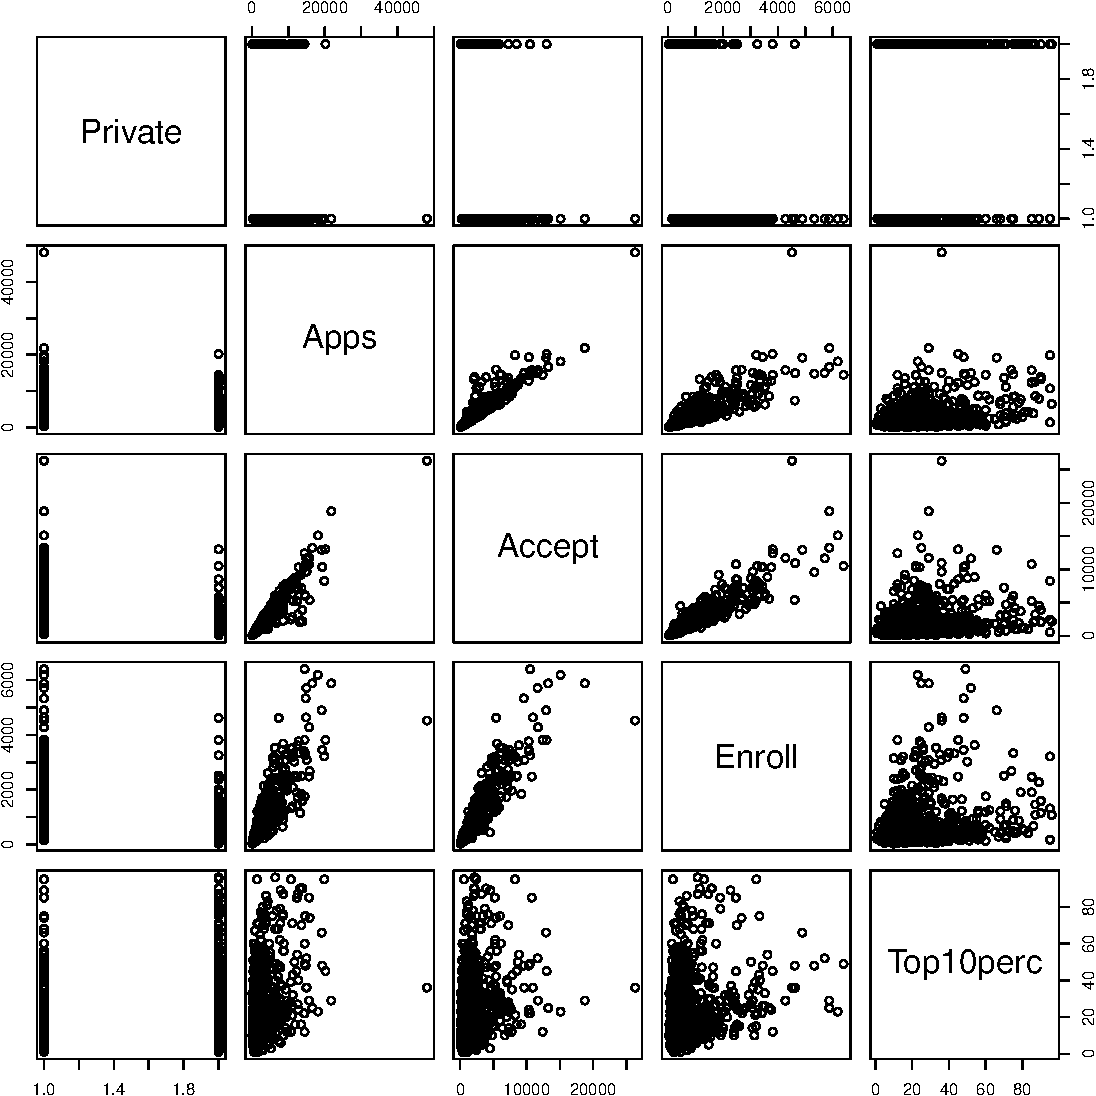
\includegraphics{Lab1Q_files/figure-latex/unnamed-chunk-5-1.pdf}

We can also look at this using the \texttt{ggpairs} function. Install
the library \texttt{GGally} if it is not available (and any dependent
libraries) and load it.

\begin{Shaded}
\begin{Highlighting}[]
\KeywordTok{library}\NormalTok{(GGally)}
\KeywordTok{ggpairs}\NormalTok{(College, }\DataTypeTok{columns=} \KeywordTok{c}\NormalTok{(}\DecValTok{1}\NormalTok{,}\DecValTok{3}\OperatorTok{:}\DecValTok{5}\NormalTok{, }\DecValTok{2}\NormalTok{))}
\end{Highlighting}
\end{Shaded}

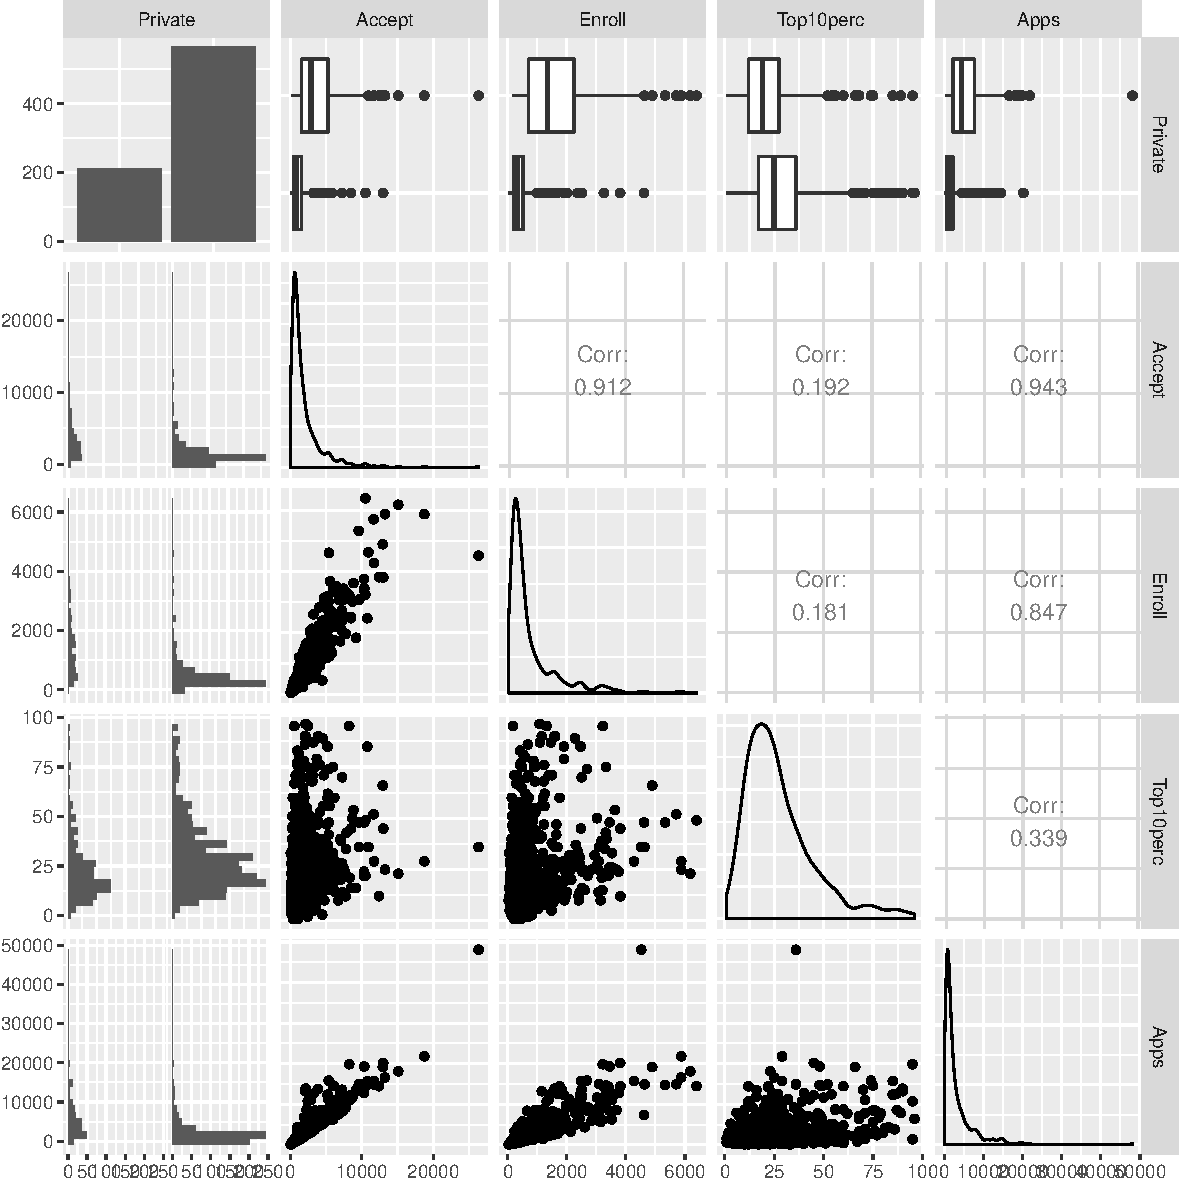
\includegraphics{Lab1Q_files/figure-latex/ggpairs-1.pdf}

The last variable \texttt{Apps} is our response. It indicates the number
of applications received.

The \texttt{ggpairs} function realizes that the variable
\texttt{Private} is categorial and plots side by side histograms. The
density plots are also useful for seeing the skewness in the marginal
distributions.

What other features do these plots indicate?

\subsubsection{New variables}\label{new-variables}

Let's create a new variable \texttt{Elite} by binning the
\texttt{Top10perc} variable. We are going to divide universities into
two groups based on whether or not the proportion of students coming
from the top 10\% of their high school classes exceeds 50\%. We will use
the library \texttt{dplyr} to illustrate some of the possible
transformations and the idea of pipes, which are quite powerful once you
get the hang of them!

\begin{Shaded}
\begin{Highlighting}[]
\KeywordTok{library}\NormalTok{(dplyr)}
\NormalTok{College =}\StringTok{ }\NormalTok{College }\OperatorTok\StringTok{ }
\StringTok{  }\KeywordTok{mutate}\NormalTok{(}\DataTypeTok{Elite =} \KeywordTok{factor}\NormalTok{(Top10perc }\OperatorTok{>}\StringTok{ }\DecValTok{50}\NormalTok{)) }\OperatorTok
\StringTok{  }\KeywordTok{mutate}\NormalTok{(}\DataTypeTok{Elite =} \KeywordTok{recode}\NormalTok{(Elite, }\StringTok{'TRUE'}\NormalTok{ =}\StringTok{ "Yes"}\NormalTok{, }\StringTok{'FALSE'}\NormalTok{ =}\StringTok{ "No"}\NormalTok{))}
\end{Highlighting}
\end{Shaded}

\emph{What is the above doing?} Document the code here.

Compare to the base \texttt{R} code:

\begin{Shaded}
\begin{Highlighting}[]
\NormalTok{Elite =}\StringTok{ }\KeywordTok{rep}\NormalTok{(}\StringTok{"No"}\NormalTok{, }\KeywordTok{nrow}\NormalTok{(College))}
\NormalTok{Elite[College}\OperatorTok{$}\NormalTok{Top10perc }\OperatorTok{>}\StringTok{ }\DecValTok{50}\NormalTok{] =}\StringTok{ "Yes"}
\NormalTok{Elite =}\StringTok{ }\KeywordTok{as.factor}\NormalTok{(Elite)}
\NormalTok{college =}\StringTok{ }\KeywordTok{data.frame}\NormalTok{(College, Elite)}
\end{Highlighting}
\end{Shaded}

\emph{How many Elite Universities are there?}

\begin{Shaded}
\begin{Highlighting}[]
\KeywordTok{summary}\NormalTok{(College}\OperatorTok{$}\NormalTok{Elite)}
\end{Highlighting}
\end{Shaded}

\begin{verbatim}
##  No Yes 
## 699  78
\end{verbatim}

\subsubsection{Side-by-side boxplots}\label{side-by-side-boxplots}

Let's plot the variable \texttt{Outstate} versus \texttt{Elite} using
side-by-side boxplots. Using \texttt{base\ R} we would enter:

\begin{Shaded}
\begin{Highlighting}[]
\KeywordTok{boxplot}\NormalTok{(Outstate }\OperatorTok{~}\StringTok{ }\NormalTok{Elite, }\DataTypeTok{data =}\NormalTok{ College, }\DataTypeTok{ylab =} \StringTok{"Outstate"}\NormalTok{, }\DataTypeTok{xlab =} \StringTok{"Elite"}\NormalTok{)}
\KeywordTok{title}\NormalTok{(}\StringTok{"Distribution of Out of State Tuition"}\NormalTok{)}
\end{Highlighting}
\end{Shaded}

\begin{center}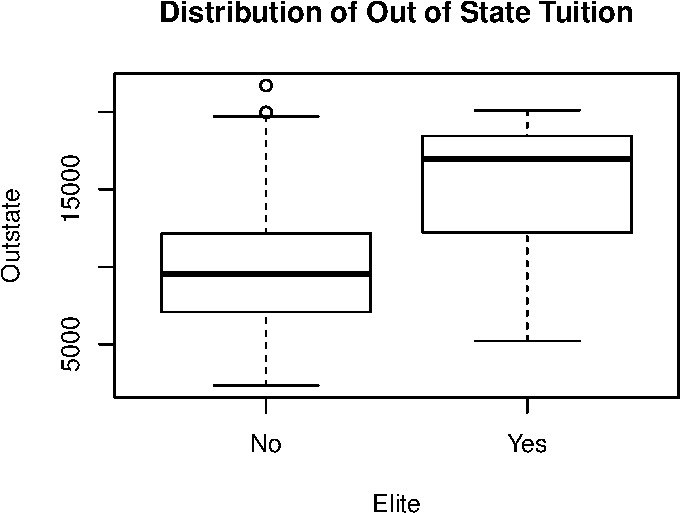
\includegraphics{Lab1Q_files/figure-latex/unnamed-chunk-9-1} \end{center}

Now for the \texttt{ggplot} version:

\begin{Shaded}
\begin{Highlighting}[]
\KeywordTok{library}\NormalTok{(ggplot2)}
\NormalTok{my.bp <-}\StringTok{ }\KeywordTok{ggplot}\NormalTok{(}\DataTypeTok{data =}\NormalTok{ College, }\KeywordTok{aes}\NormalTok{(}\DataTypeTok{y =}\NormalTok{ Outstate, }\DataTypeTok{x =}\NormalTok{ Elite)) }\CommentTok{# Creates boxplots}
\NormalTok{my.bp <-}\StringTok{ }\NormalTok{my.bp }\OperatorTok{+}\StringTok{ }\KeywordTok{geom_boxplot}\NormalTok{() }\CommentTok{# Adds color}
\NormalTok{my.bp <-}\StringTok{ }\NormalTok{my.bp }\OperatorTok{+}\StringTok{ }\KeywordTok{ggtitle}\NormalTok{(}\StringTok{"Distribution of Out of State Tuition"}\NormalTok{) }\CommentTok{# Adds a title}
\NormalTok{my.bp <-}\StringTok{ }\NormalTok{my.bp }\OperatorTok{+}\StringTok{  }\KeywordTok{ylab}\NormalTok{(}\StringTok{"Outstate"}\NormalTok{) }\OperatorTok{+}\StringTok{ }\KeywordTok{xlab}\NormalTok{(}\StringTok{"Elite"}\NormalTok{) }\CommentTok{# Adds lables for axes}
\NormalTok{my.bp }\CommentTok{# displays the boxplots}
\end{Highlighting}
\end{Shaded}

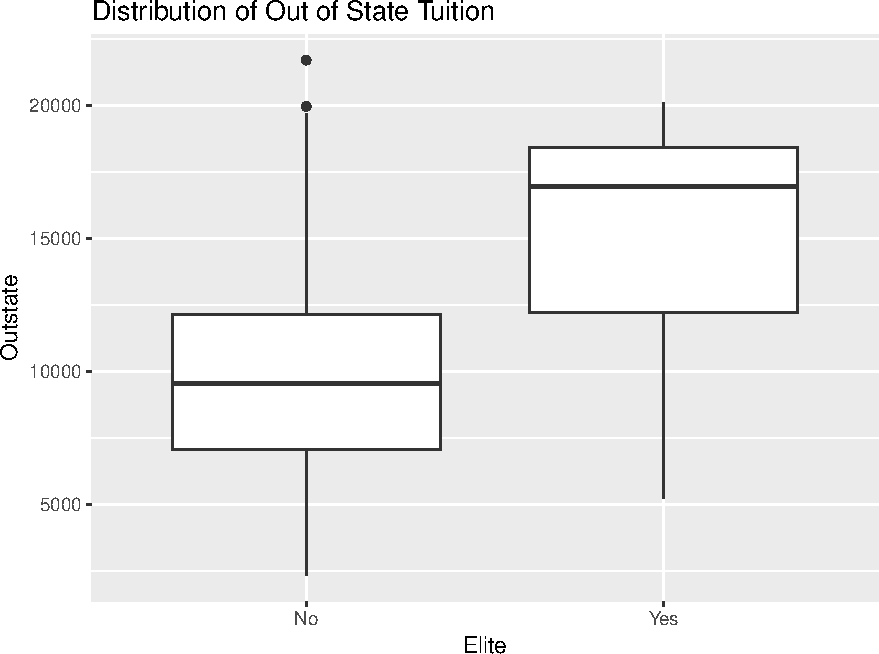
\includegraphics{Lab1Q_files/figure-latex/unnamed-chunk-10-1.pdf}

\subsubsection{Conditional Plots}\label{conditional-plots}

Let's look at the distribution of out of state tuition
(\texttt{Outstate}) versus Elite status for Private versus Public
universities using \emph{conditional plots}

\begin{Shaded}
\begin{Highlighting}[]
\KeywordTok{coplot}\NormalTok{(Outstate }\OperatorTok{~}\StringTok{ }\NormalTok{Elite }\OperatorTok{|}\StringTok{ }\NormalTok{Private, }\DataTypeTok{data =}\NormalTok{ College)}
\end{Highlighting}
\end{Shaded}

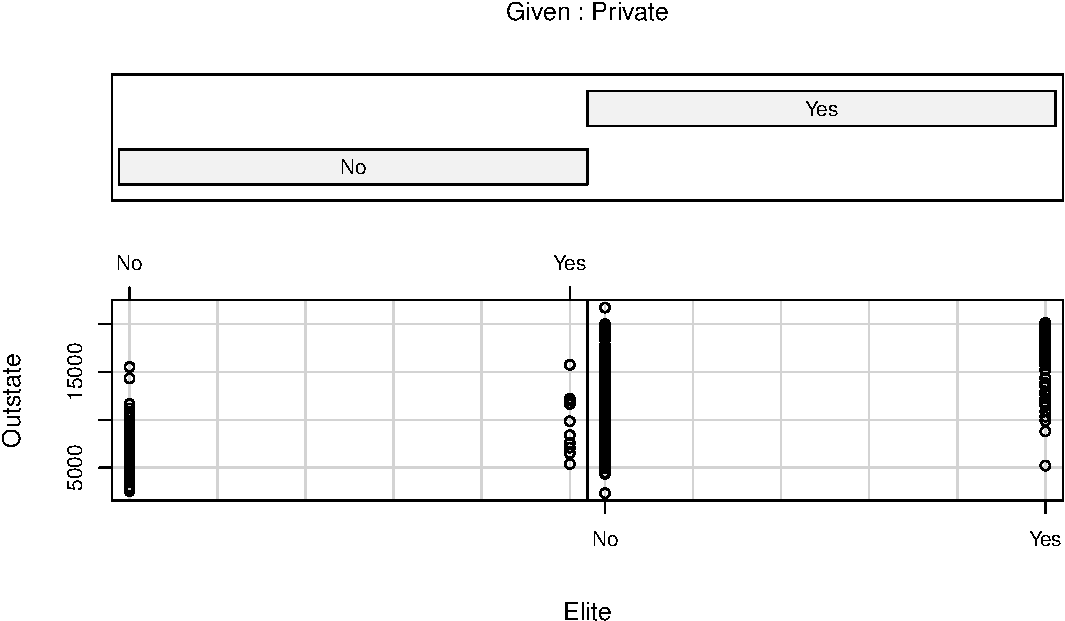
\includegraphics{Lab1Q_files/figure-latex/unnamed-chunk-11-1.pdf}

\subsection{ggplot conditional plot}\label{ggplot-conditional-plot}

\begin{Shaded}
\begin{Highlighting}[]
\KeywordTok{library}\NormalTok{(ggplot2)}
\KeywordTok{ggplot}\NormalTok{(College, }\KeywordTok{aes}\NormalTok{(}\DataTypeTok{x =}\NormalTok{ Elite, }\DataTypeTok{y =}\NormalTok{ Outstate, }
                    \DataTypeTok{group =}\NormalTok{ Private, }
                    \DataTypeTok{color =}\NormalTok{ Private)) }\OperatorTok{+}
\StringTok{   }\KeywordTok{geom_point}\NormalTok{() }\OperatorTok{+}\StringTok{ }\KeywordTok{facet_grid}\NormalTok{(.}\OperatorTok{~}\NormalTok{Private) }\OperatorTok{+}\StringTok{ }\KeywordTok{ggtitle}\NormalTok{(}\StringTok{"Distribution of Out of State Tuition"}\NormalTok{) }
\end{Highlighting}
\end{Shaded}

\begin{center}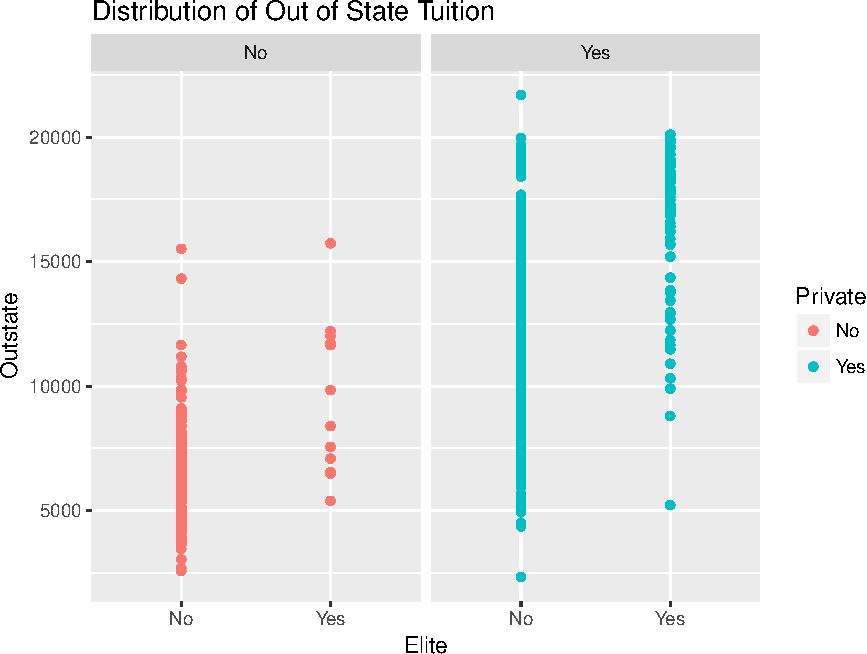
\includegraphics{Lab1Q_files/figure-latex/unnamed-chunk-12-1} \end{center}

\subsection{Next Steps}\label{next-steps}

Update this document and explore the other variables thinking about the
objective of predicting \texttt{Apps}. Document what you discover
thinking about models to predict \texttt{Apps}.

\section{\texorpdfstring{On your own: the \texttt{Auto}
dataset}{On your own: the Auto dataset}}\label{on-your-own-the-auto-dataset}

The \texttt{Auto} dataset is a data frame with 392 observations on the
following 9 variables:

\begin{itemize}
\tightlist
\item
  \texttt{mpg} : miles per gallon
\item
  \texttt{cylinders}: number of cylinders between 4 and 8
\item
  \texttt{displacement}: engine displacement (cu. inches)
\item
  \texttt{horsepower}: engine horsepower
\item
  \texttt{weight}: vehicle weight (lbs.)
\item
  \texttt{acceleration}: time to accelerate from 0 to 60 mph (sec.)
\item
  \texttt{year}: model year (modulo 100)
\item
  \texttt{origin}: origin of car (1. American, 2. European, 3. Japanese)
\item
  \texttt{name}: vehicle name
\end{itemize}

This dataset was taken from the StatLib library which is maintained at
Carnegie Mellon University. The dataset was used in the 1983 American
Statistical Association Exposition. The dataset is available with the
ISLR library.

Load the data and answer the following questions adding your code in the
code chunks.

\begin{enumerate}
\def\labelenumi{\arabic{enumi}.}
\item
  Create a summary of the data. How many variables have missing data?
\item
  Which of the predictors are quantitative, and which are qualitative?
\item
  What is the range of each quantitative predictor? You can answer this
  using the \texttt{range()} function. Create a table with variable
  name, min, max with one row per variable. \texttt{kable} from the
  package \texttt{knitr} can display tables nicely.
\item
  What is the mean and standard deviation of each quantitative
  predictor? \emph{Format nicely in a table as above}
\item
  Now remove the 10th through 85th observations (try this with
  \texttt{filter} from the \texttt{dplyr} package). What is the range,
  mean, and standard deviation of each predictor in the subset of the
  data that remains? \emph{Again, present the output as a nicely
  formatted table}
\item
  Investigate the predictors graphically, using scatterplot matrices
  (\texttt{ggpairs}) and other tools of your choice. Create some plots
  highlighting the relationships among the predictors. Comment on your
  findings. \emph{Try adding a caption to your figure}
\item
  Suppose that we wish to predict gas mileage (\texttt{mpg}) on the
  basis of the other variables using regression. Do your plots suggest
  that any of the other variables might be useful in predicting mpg
  using linear regression? Justify your answer.
\end{enumerate}


\end{document}
